\section{Three regimes}\label{sec:regimes}

\begin{quote}
\textbf{In plain words.} Close to a moving magnet, a compass needle follows it
at once; far away, all that is left is a radio wave, fading with distance. These
are the \href{https://en.wikipedia.org/wiki/Near_and_far_field}{near field and
the far field}, and gravity has the same two, divided at about a sixth of a
wavelength from the source (the wavelength over $2\pi$). A body that moves once
a second would radiate waves $300{,}000\,\mathrm{km}$ long, so its near zone
reaches $48{,}000\,\mathrm{km}$. Everyday life happens in the near field.

Matter radiates in two ways: bodies in bulk motion at the low frequencies at
which they move, and hot matter at the very high frequencies at which its
molecules jostle. The camera therefore has three regimes: the near field, where
it sees the changing pull of mass and the image blurs with distance; waves from
moving bodies, in which a compact source is a point; and the thermal glow, which
could be sharp but is so faint that almost no
\href{https://en.wikipedia.org/wiki/Graviton}{gravitons} arrive. Three facts
explain most of what follows. Gravity has
\href{https://en.wikipedia.org/wiki/Spin_(physics)}{spin} two, so its field at a
point is a pattern of stretch and squeeze, not an arrow like that of light;
matter moves slowly compared with light; and matter is too spread out, its ratio
$GM/Rc^2$ tiny, to bend or block gravity's waves short of a black hole.
\end{quote}

What reaches a pixel depends on how the distance $r$ to the source compares
with the wavelength $\lambda = c/f$ of the radiation it would emit at frequency
$f$. Inside the \emph{near zone},
\begin{equation}\label{eq:nearzone}
r \ll \frac{\lambda}{2\pi} = \frac{c}{2\pi f},
\end{equation}
the field is the Newtonian one of Eq.~\eqref{eq:newton}, following the source
almost instantaneously. Outside it the field is radiation, Eq.~\eqref{eq:wave},
falling off as $1/r$. At $1\,\mathrm{Hz}$ the near zone reaches to
$48{,}000\,\mathrm{km}$; at $1\,\mathrm{kHz}$, to $48\,\mathrm{km}$.
Figure~\ref{fig:regimes} places familiar sources on this map.

\begin{figure}
\centering
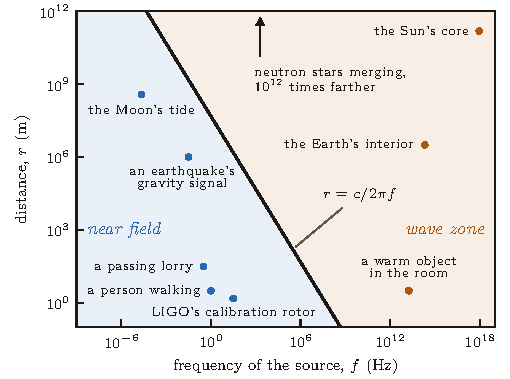
\includegraphics[width=\columnwidth]{figures/regimes.pdf}
\caption{Where sources lie. The diagonal is the edge of the near zone,
Eq.~\eqref{eq:nearzone}, $r = c/2\pi f$. Everything that moves mechanically,
from the tides to a calibration rotor beside a LIGO mirror, sits below it and
is seen through its changing Newtonian pull. Only radiation at thermal
frequencies, far to the right, reaches a nearby camera as waves short enough to
form sharp images; thermal sources are placed at the peak of their spectrum,
$f = 2.82\,k_BT/2\pi\hbar$.}\label{fig:regimes}
\end{figure}

Sources of radiation divide again. Bodies in bulk motion radiate at the
frequencies at which they move, which are low; hot matter radiates at the
frequencies of its molecular motion, which are very high. This gives the three
regimes of Table~\ref{tab:regimes}, taken in turn in the next three sections.

\paragraph{Spin, speed and compactness.} Almost everything the camera can and
cannot do follows from one property of gravity and two small numbers that
describe matter. \emph{Gravity has spin two}: curvature at a point is
a symmetric trace-free tensor, and in a wave it is the square
$\mathbf m\mathbf m^T$ of a complex null vector $\mathbf m$, where the field of
light is the vector itself. This gives the ten numbers of a pixel, the four
principal null directions of a reading, the separation of two, three and four
waves, the sixty-eight numbers of the sky that one pixel can measure and the
spin-two envelope of a sparse array (Section~\ref{sec:one-pixel}). \emph{Matter is slow},
$v/c \ll 1$: this puts the edge of the near zone, $\lambda/2\pi \sim L/(v/c)$,
far beyond any room, makes every compact moving body a point in its own
radiation (Section~\ref{sec:waves}), and makes the magnetic part of a near field
small, so that it is at once a clean channel for waves and a range-finder for
moving mass; only thermal motion reaches the frequencies at which the
wavelength is shorter than the body. \emph{Matter is tenuous}, its compactness
$GM/Rc^2 \ll 1$: this makes it transparent, so that hot matter glows
throughout (Section~\ref{sec:thermal}), and rules out lenses, mirrors,
absorbers and shadows short of a black hole (Section~\ref{sec:no-lens}), so
that images must be computed.

\begin{table}
\centering
\begin{tabular}{p{0.26\linewidth}p{0.4\linewidth}p{0.22\linewidth}}
Regime & What the pixel receives & What limits the image \\ \hline
Near field & the changing Newtonian pull of nearby mass & blur grows with distance \\
Waves from bulk motion & radiation from accelerating bodies & a compact source is an unresolved point \\
Thermal glow & radiation from molecular motion & almost no gravitons arrive \\
\end{tabular}
\caption{The three regimes of a gravitational camera.}\label{tab:regimes}
\end{table}
